%!TEX root = ./../springer-mono-format/book.tex
%!TEX root = ./../thesis-trier.tex

\chapter{Short Introduction to Synchronizing Automata}
\label{intro:chap:short_intro_sync_aut}
\label{intro:aut_and_formal_lang}

%!TEX root = ./../../springer-mono-format/book.tex
%!TEX root = ./../../thesis-trier.tex

This chapter gives a short introduction to synchronizing automata for readers unfamiliar with the topic. \Cref{intro:sec:basic} fixes the notation needed here. The notation for the
remainder of the thesis is given in~\cref{chap:prelim}.
In \cref{intro:sec:defsyncaut} 
we formally introduce synchronizing automata. Then, in~\cref{intro:sec:examples}, we present several introductory examples and 
problems and discuss their relation to synchronizing automata.
Finally,
\cref{intro:sec:cerny} defines the reset length, states \Cerny's conjecture,
and presents the \Cerny automata, which serve as a running example throughout
the thesis.

For readers who want to learn more about synchronizing automata, the most recent survey articles are by Kari and Volkov~\cite{KariVolkov2021} (see also its precursor~\cite{DBLP:conf/lata/Volkov08}) and by Volkov~\cite{Volkov22}, 
the latter containing a good coverage
of applications from different fields and types of automata considered in the literature.
 The surveys by Jürgensen~\cite{DBLP:journals/iandc/Jurgensen08}, Kari and Volkov~\cite{KariVolkov2021}, and Béal and Perrin~\cite{BealPerrin2016} discuss connections to codes (see also Chapters~3 and~10 of~\cite{DBLP:books/daglib/0025093}). Sandberg~\cite{Sandberg04} and Kohavi~\cite[Chap.~13]{Kohavi70} include relations to automata with outputs as well as applications in circuit theory and testing. The survey by Bogdanović et al.~\cite{Bogdanovic99} presents structural results not covered in the other surveys. Another survey is by Mateescu and Salomaa~\cite{MateescuS01}. Finally, we recommend~\cite{ArCamSt2017} on synchronizing permutation groups, motivated by synchronizing automata, as results presented in that survey were inspirational for our results in \cref{sync_max:sec:perm_grps} from \cref{part:aut}.

\section{Notions Used in the Introduction}
\label{intro:sec:basic}

%!TEX root = ./../../springer-mono-format/book.tex
%!TEX root = ./../../thesis-trier.tex

\IN{cardinality}
\IN{set membership}
If $X$
is a set, by $|X|$ we denote its \emph{cardinality}  and $x \in X$ denotes \emph{set membership}, i.e., the fact that $x$
is an element in $X$. 
We use standard \emph{set builder notation} $\{ x \mid P(x)\}$ 
or 
$\{ x : P(x)\}$ for the set of all elements $x$ satisfying a predicate $P(x)$.
%\footnote{We prefer $\mid$, but use ''$:$'' in case $P$ involves
	%starts with a vertical bar.}
The \emph{empty set} is denoted by $\emptyset$. 
For sets $X,Y$, we write $f \colon X \to Y$
for a \emph{(total) function} (also called a \emph{map} or \emph{mapping}) with \emph{domain} $X$ and 
\emph{codomain} $Y$, assigning to each $x \in X$ an element $\applyfunc{x}{f} \in Y$.
\label{def:emptyset}
\label{def:function-application}
\IN{empty set}
\IN{set builder notation}
\label{def:total_function}


\IN{domain!of function}
\IN{codomain!of function}
\IN{function}
\index{total function|see{function}}
\index{map|see{function}}
\label{def:n-times-concat}
\IN{concatenation product}
\index{language|see{formal language (over $\Sigma$)}}
\IN{formal language (over $\Sigma$)}
\IN{empty word}
\label{def:Sigmastar}
\index{finite alphabet|see{alphabet}} 
\IN{alphabet} 
\IN{symbol} 
\index{letter|see{symbol}}
\label{def:Sigma}
\IN{word}
\IN{length of word}
\label{def:length_of_word}
\label{def:empty-word} 
Let $\Sigma$ denote a \emph{finite alphabet}, i.e., a set of \emph{symbols} or \emph{letters} (we always use $\Sigma$ to denote an alphabet in the present work). 
A \emph{word (over $\Sigma$)}, also called a \emph{string}, is a finite sequence of elements from~$\Sigma$.
By $\Sigma^*$ we denote the \emph{set of all words} over $\Sigma$.
We identify each symbol in $\Sigma$ with the corresponding word of length one. In this way, we have $\Sigma \subseteq \Sigma^*$.
For $u,v \in \Sigma^*$ we write $u\cdot v$, or $uv$ for short, for the \emph{concatenation (product)} of both words.\footnote{For a more formal	construction of $\Sigma^*$ and concatenation, see, for example, the textbook~\cite[p.~5]{Eilenberg1974}.}
We denote the \emph{length} of $u \in \Sigma^*$ by~$|u|$. 
The \emph{empty word}, i.e., the word of length zero,  
is denoted by $\varepsilon$. For $u \in \Sigma^*$, we set $u^0 = \varepsilon$ and $u^n = u\cdots u$ ($n$ times) for $n > 0$. 
Subsets of $\Sigma^*$ are called \emph{(formal) languages (over $\Sigma$)}. 

\IN{natural numbers} 
\label{def:N0} 
\label{def:finite_set_n}  
\label{def:min} 
\label{def:max} 
By $\mathbb N_0 = \{ 0,1,2,\ldots \}$
we denote the \emph{set of natural numbers}, including zero,
with the usual orders $\le$ and $<$ on $\mathbb N_0$.
For $n \in \mathbb N_0$ we set $[n] = \{ m \in \mathbb N_0 \mid m < n \}$.
For a non-empty  subset $M$ of $\mathbb N_0$, 
by $\min(M)$, or $\min M$ for short, (resp.~$\max(M)$, or $\max M$, for finite $M$) 
we denote the \emph{smallest} (resp.~\emph{largest}) \emph{number} in~$M$ w.r.t.~the usual order.
We also set $\min(a_1, \ldots, a_n) = \min\{a_1, \ldots, a_n\}$ (resp.~$\max(a_1, \ldots, a_n) = \max\{a_1, \ldots,a_n\}$)
for $a_1, \ldots, a_n \in \mathbb N_0$ with $n \ge 1$.
We also denote the integers and the real numbers by $\mathbb Z$ and $\mathbb R$, respectively.
\IN{real numbers}
\IN{integers}
\label{def:integers}
\label{def:realnumbers}

\label{def:automaton}
\index{deterministic and complete finite automaton|see{deterministic and complete finite semiautomaton}}
\index{automaton|see{deterministic and complete finite semiautomaton}}
\index{semiautomaton|see{deterministic and complete finite semiautomaton}}
\IN{deterministic and complete finite semiautomaton}
\IN{state set!of an automaton} 
\IN{input alphabet!of an automaton}
\IN{transition function!of an automaton}
\index{finite state set|see{state set}} 
\IN{image of subset!of transition function} % attribute/adjective/modifier
A \emph{(deterministic and complete) finite semiautomaton} over~$\Sigma$ (or just \emph{automaton} for short) is a tuple $\semiautomat{A}{Q}{\Sigma}{\delta}$
where $Q$ is the \emph{finite state set}, $\Sigma$ the \emph{finite input alphabet},
and $\delta \colon Q \times \Sigma \to Q$ the \emph{(totally defined) transition function}.\footnote{\emph{Deterministic} means that $\delta$ is a function rather than a
	relation, and \emph{complete} means that it is total. Both modifiers are
	redundant here, as we consider no other kind of automaton, but we state
	them as a reminder for readers used to the nondeterministic setting. In
	\cref{part:constrsync}, we also introduce partial automata, where the
	transition function may be partially defined.%	
	}
We extend $\delta$ to a function $\hat\delta \colon Q \times \Sigma^* \to Q$
by setting $\applytrans{\hat\delta}{q}{\varepsilon} = q$
and $\applytrans{\hat\delta}{q}{ux} = \applytrans{\delta}{\applytrans{\hat\delta}{q}{u}}{x}$
for $q \in Q$, $u \in \Sigma^*$, and $x \in \Sigma$. For simplicity, we denote the extension $\hat\delta$ 
by $\delta$ as well. Given $S \subseteq Q$ and~$u \in \Sigma^*$ the \emph{image (of $S$ under $u$)} is $\applytrans{\delta}{S}{u} = \{ \applytrans{\delta}{q}{u} \mid q \in S \}$. 
\label{def:image-delta}

\IN{state diagram}
Automata are often specified graphically as \emph{state diagrams}, where states are represented as points or circles, and a transition $\delta(p, a) = q$ for $p, q \in Q$ and $a \in \Sigma$ is depicted by an arrow from $p$ to $q$ labeled by $a$. Multiple transitions between the same pair of states are typically combined into a single arrow labeled with the corresponding set of input symbols. See \cref{intro:ex:automaton} for an example of an automaton together with its state diagram.

\begin{example} \label{intro:ex:automaton}
	Consider \cref{intro:fig:cernyfour} for the state diagram
	of the automaton $\semiautomat{A}{Q}{\Sigma}{\delta}$
	with state set $Q = \{0,1,2,3\}$,
	two letters $\Sigma = \{a,b\}$ and where $\delta \colon Q \times \Sigma \to Q$
	is given by $\delta(q, b) = q + 1$ for $q \in \{0,1,2\}$, $\delta(3, b) = 0$,
	$\delta(0, a) = 1$, and $\delta(q, a) = q$ for $q \in \{1,2,3\}$.
\end{example}

\begin{figure}[ht]
	\centering
	\begin{tikzpicture}[shorten >=1pt,->,node distance=2.3cm]
		\node[state] (0) {$0$};
		\node[state, right of=0] (1) {$1$};
		\node[state, below of=1] (2) {$2$};
		\node[state, left of=2]  (3) {$3$};
		
		\path[->] (0) edge [above] node {$a,b$} (1)
		(1) edge [right] node {$b$} (2)
		(2) edge [loop right] node {$a$} (2)
		(2) edge [below] node {$b$} (3)
		(3) edge [left]  node {$b$} (0)
		(2) edge [loop right] node {$a$} (2)
		(3) edge [loop left]  node {$a$} (3)
		(1) edge [loop right] node {$a$} (1);
	\end{tikzpicture}
	\caption[Example automaton]{The state diagram of the automaton from \cref{intro:ex:automaton}.}
	\label{intro:fig:cernyfour}
\end{figure}	

\section{Formal Definition of Automata Synchronization}
\label{intro:sec:defsyncaut}

%!TEX root = ./../../springer-mono-format/book.tex

\label{def:set_of_sync_words} 
\IN{synchronizing word} \index{reset word|see{synchronizing word}}
\IN{synchronizing word} 
\IN{set of synchronizing words}
\IN{synchronizing automaton}
\IN{synchronizing state}
An automaton $\semiautomat{A}{Q}{\Sigma}{\delta}$ 
is \emph{synchronizing} (or \emph{resettable})
if there exists a word, called a \emph{reset} or \emph{synchronizing word},
driving it into the same state regardless of its current state. 
Formally, a word $u \in \Sigma^*$ is said to be a \emph{synchronizing} (or \emph{reset}) \emph{word} for~$\mathcal A$
if $\applytrans{\delta}{Q}{u} = \{q\}$ for some $q \in Q$.
In this case, 
we say that $u$ \emph{synchronizes} $\mathcal A$, and that~$q$ is a \emph{synchronizing state} of $\mathcal A$.
The \emph{set of synchronizing words} of~$\mathcal A$
is denoted by $\Syn(\mathcal A) = \{ u \in \Sigma^* \mid \exists q \in Q \colon \delta(Q, u) = \{q\} \}$.
Then $\mathcal A$ is synchronizing if and only if $\Syn(\mathcal A)$ is non-empty.

Synchronizing words
correspond to a sequence of actions (or inputs) that
allow an operator (or observer) to regain
control by resetting the automaton into a well-defined state.
This notion arises in different contexts and applications
in coding theory~\cite{DBLP:books/daglib/0025093,DBLP:journals/iandc/Jurgensen08,KariVolkov2021}, robotics~\cite{Eppstein90,DBLP:journals/algorithmica/Goldberg93,DBLP:conf/focs/Natarajan86,DBLP:conf/lata/Volkov08}, 
symbolic dynamics~\cite{trahtman09}, model checking and verification~\cite{Sandberg04}, and group theory~\cite{ArCamSt2017}.

The introduction of synchronizing automata is often attributed to \Cerny and
his seminal paper~\cite{Cer64}. However, the actual history is more complicated
and the concept can be traced back to earlier work of Laemmel~\cite{Laemmel63}
and Liu~\cite{Liu63}.
For a detailed account on the genesis of this concept,
see the survey~\cite[Sect.~1.3]{Volkov22}.	

\section{Introductory Examples}
\label{intro:sec:examples}

%!TEX root = ./../../springer-mono-format/book.tex
%!TEX root = ./../../thesis-trier.tex

Here,  we introduce several situations and problems
which can be modeled using synchronizing automata:
a problem from coding theory in \cref{intro:sec:examples:communication},
a puzzle from Ashby in \cref{intro:sec:examples:puzzle},
a conveyor belt and part orienter design problem in \cref{intro:sec:examples:partorienters},
and a maze orientation problem in \cref{intro:sec:examples:maze}.

\subsection{Error-Prone Communication Channels}
\label{intro:sec:examples:communication}

Suppose five symbols $e,h,l,o,r$ are encoded by five binary sequences $00$, $01$, $10$, $110$,
and $111$, respectively, see \cref{fig:intro:encoding}. This coding scheme is taken from Neumann~\cite{neumann71}. 

\begin{figure}[t]
	\centering
	\begin{subfigure}[b]{.38\textwidth}
		\centering
		\[
		\begin{array}{c|c}
			\text{Symbol} & \text{Binary Encoding} \\ \hline 
			e & 00 \\
			h & 01 \\
			l & 10 \\
			o & 110 \\
			r & 111
		\end{array} 
		\]
		\caption{Encoding of source symbols.}
		\label{intro:fig:decoder:code}
	\end{subfigure}%
	\hfill
	\begin{subfigure}[b]{0.6\textwidth}
		\centering
		\begin{tikzpicture}[shorten >=1pt,node distance=1.5cm and 1cm,on grid,auto,font=\sffamily] 
			\node (eps)  {$\varepsilon$};
			\node (0) [xshift=-0.7cm,  below left=of eps]  {$0$};
			\node (1) [xshift=0.7cm, below right=of eps] {$1$};
			\node (11) [below right=of 1]  {$11$};
			\node (00)  [below left = of 0]   {$00$};
			\node (01)  [below right = of 0]  {$01$};
			\node (110) [below left = of 11]  {$110$};
			\node (111) [below right = of 11] {$111$};
			\node (10)  [below left = of 1] {$10$};
			
			\path[->] (eps) edge [dashed] node {} (0)
			(eps) edge node {} (1)
			(1)   edge node {} (11)
			(0)   edge [dashed] node {} (00)
			(0)   edge node {} (01)
			(11)  edge [dashed] node {} (110)
			(11)  edge node {} (111)
			(1)   edge [dashed] node {} (10);
			
			\node (e) [yshift=0.9cm, below = of 00] {$e$};
			\node (h) [yshift=0.9cm, below = of 01] {$h$};
			\node (l) [yshift=0.9cm, below = of 10] {$l$};
			\node (o) [yshift=0.9cm, below = of 110] {$o$};
			\node (r) [yshift=0.9cm, below = of 111] {$r$};
		\end{tikzpicture}
		\caption{Decision tree to decode symbols for binary inputs where dashed and solid branches correspond to $0$ and $1$, respectively.}
		\label{fig:tree-encoding}
	\end{subfigure}
	\caption{Encoding of five symbols $e$, $h$, $l$, $o$, and~$r$  by binary sequences.}
	\label{fig:intro:encoding}
\end{figure}

When transmitting a message using this code, is it possible to recover from a loss of synchronization between the sender (encoder) and receiver (decoder) caused by channel errors?
For example, suppose the sender wants to transmit ``hello'' 
to the receiver, which corresponds to the bit sequence ``$01\ 00\ 10\ 10\ 110$''. However, after sending the first three bits, the sender is uncertain whether they were received correctly.

On the receiving end, a stream of code words can be decoded with the help of the automaton 
shown in \cref{intro:subfig:decoder},
which starts in the state~$q_{\varepsilon}$ and reflects different states of the receiver.
A path starting in~$q_{\varepsilon}$ and going back to~$q_{\varepsilon}$
corresponds to a received code word, 
where the transition leading into~$q_{\varepsilon}$
indicates which code word was received.
For example, when reading ``$01\ 00\ 10\ 10\ 110$'', starting from $q_{\varepsilon}$,
the transitions returning to $q_{\varepsilon}$ indicate the sequence ``hello'' in that order. 

\begin{figure}[ht]
	\centering
	\begin{subfigure}[b]{.6\textwidth}
		\centering
			\begin{tikzpicture}[shorten >=1pt,node distance=3cm,on grid,auto,font=\sffamily] 
				\node[state,blur shadow,fill={rgb:black,0.4;white,10}] (eps)  {$q_{\varepsilon}$};
				\node[state,blur shadow,fill={rgb:black,0.4;white,10}] (0) [below left=of eps]  {$q_{0}$};
				\node[state,blur shadow,fill={rgb:black,0.4;white,10}] (1) [xshift=-0.3cm, yshift=0.3cm, below right=of eps] {$q_{1}$};
				\node[state,blur shadow,fill={rgb:black,0.4;white,10}] (11) [xshift=-0.7cm, yshift=0.7cm,below right=of 1]  {$q_{11}$};
				
				\path[->] (eps) edge [dashed] node {} (0)
				(eps) edge node {} (1)
				(1)   edge node {} (11)
				(0)   edge [dashed,out=90,in=190, below, pos=.7] node {$e$} (eps)
				(0)   edge [out=130,in=150,pos=.7] node {$h$} (eps)
				(1)   edge [dashed,out=180, in=280, above] node {$l$} (eps)
				(11)  edge [dashed,out=190, in=270, pos=.8] node {$o$} (eps)
				(11)  edge [out=80, in=0, above, pos=0.8] node {$r$} (eps);
		\end{tikzpicture}
		\caption{Starting from $q_{\varepsilon}$, each return to $q_{\varepsilon}$ 
			corresponds to the decoding of one code word; the label on the return transition indicates the decoded source symbol.
		}
	\label{intro:subfig:decoder}	
\end{subfigure}%
\hfill
\begin{subfigure}[b]{0.35\textwidth}
	\centering
	\[
	\begin{array}{l|lllll}
		& 0 & 1 & 1 & 0 \\ \hline       
		q_{\varepsilon} & q_0 & q_{\varepsilon} & q_1 & q_{\varepsilon}  \\
		q_{0}           & q_{\varepsilon} & q_{1} & q_{11} & q_{\varepsilon} \\
		q_1             & q_{\varepsilon} & q_1   & q_{11} & q_{\varepsilon} \\
		q_{11}          & q_{\varepsilon} & q_1   & q_{11} & q_{\varepsilon}
	\end{array}
	\]
	\caption{The state transitions for the input sequence $0110$ starting from each state.}
	\label{intro:fig:decoder:syncsequence}
\end{subfigure}
\caption[Introductory decoder automaton]{Decoder automaton (left) 
	for the code from \cref{fig:intro:encoding}
	where dashed (resp. solid) transitions represent input symbol $0$ (resp. $1$)
	with the synchronizing word $0110$ (right).} 
\label{intro:fig:decoder}	
\end{figure}

Now suppose that the current state of the decoder automaton is unknown. This raises the following question.

\smallskip
\begin{center}
	\fbox{%
		\begin{minipage}{29em}
			Can the sender transmit a sequence of bits that guarantees the receiver
			is brought to the well-defined state $q_{\varepsilon}$ in \cref{intro:subfig:decoder},
			from which it can correctly decode the next code word?
		\end{minipage}
	}
\end{center}
\smallskip

The answer is positive: as shown in \cref{intro:fig:decoder:syncsequence},
reading the sequence~$0110$ from any state of the automaton leads to $q_{\varepsilon}$.
Thus, by transmitting~$0110$, the sender can reset the receiver in case it has lost synchronization 
with the stream of code words due to errors, ensuring correct decoding of subsequent bits.

Applied to the situation above, where the sender wants to transmit ``hello'' but is unsure
whether the first three bits were transmitted correctly, the sender can send the message
\[
\underbrace{010}_{\text{uncertain bits}}
0110\,01\,00\,10\,10\,110.
\]

After reading “$010\ 0110$”,
the automaton is in the state $q_{\varepsilon}$, from which it can correctly decode the
next code word.

\subsection{The Haunted Mansion} 
\label{intro:sec:examples:puzzle}
	
Ashby~\cite{ashby_56} presented the following puzzle. A mansion is haunted
by two ghostly noises, Singing and Laughter. 
Each of the noises can independently be either on or off, and they can be influenced
by two possible actions, organ playing or burning incense, according
to the following scheme described by Ashby~\cite[pp.~60--61]{ashby_56}.

\begin{quote} 
The Singing, in the succeeding minute, will go on as it was during the preceding minute (sounding
or silent) unless there was organ-playing with no Laughter, in which case it will change to the opposite (sounding
to silent, or vice versa).

As for the Laughter, if there was incense burning, then it will sound or not according as the Singing was sounding
or not (so that the Laughter copies the Singing a minute later).
If however there was no incense burning, the Laughter will do the opposite of what the Singing did. 
\end{quote} 

The puzzle asks for a sequence of actions that silences both noises when they are both active. However, more is possible: as we shall see, there exists a sequence of actions that leads to both noises becoming silent in every possible situation.

\IN{Ashby's ghost taming automaton}
\begin{figure}[htb]
\centering
\scalebox{0.9}{
\begin{tikzpicture}[
	node distance=14em and 14em,
	on grid,
	auto,
	font=\sffamily,
	>=Stealth,
	shorten >=1pt,
	semithick
	]
	
	\node[state] (00) {$(\overline S, \overline L)$}; 
	\node[state] (01) [right=of 00] {$(\overline S, L)$};
	\node[state] (10) [below=of 01] {$(S, \overline L)$};
	\node[state] (11) [left=of 10] {$(S, L)$};
	
	\path
	(00) edge [loop left] node {$a_{\overline O B}$} (00)
	(00) edge [bend left=11] node {$a_{\overline O \overline B}$} (01)
	(00) edge [bend left=11] node {$a_{O B}$} (10)
	(00) edge [bend right=11] node[left] {$a_{O \overline B}$} (11)
	
	(01) edge [loop right] node {$a_{O\overline B}, a_{\overline O \overline B}$} (01)
	(01) edge [bend left=11] node {$a_{OB}, a_{\overline O B}$} (00)
	
	(10) edge [loop right] node {$a_{\overline O\overline B}$} (10)
	(10) edge [bend left=11] node {$a_{\overline O B}$} (11)
	(10) edge [bend left=11] node {$a_{O \overline B}$} (00)
	(10) edge [bend right=11] node[right] {$a_{OB}$} (01)
	
	(11) edge [loop left] node {$a_{\overline O B}, a_{OB}$} (11)
	(11) edge [bend left=15] node {$a_{O \overline B}, a_{\overline O \overline B}$} (10);
\end{tikzpicture}
}
\caption[Ashby's ghost taming automaton]{Ashby's ghost taming automaton. 
	The word $a_{\overline O \overline B} a_{O \overline B} a_{\overline O  B}$	is synchronizing.}
\label{intro:fig:ashby}
\end{figure} 

We can model the situation 
by an automaton $\semiautomat{A}{Q}{\Sigma}{\delta}$ with
state set 
\[
Q = \{ (S, L), (\overline S, L), (\overline S, \overline L), (S, \overline L) \},
\]
where $S$ and $\overline S$ represent the presence and absence of singing, respectively, 
and similarly for $L$ and $\overline L$ with laughter.
Furthermore, the input alphabet is 
$ \Sigma = \{ a_{OB}, a_{\overline O B}, a_{\overline O \overline B}, a_{O \overline B}\}
$
where the symbols represent the four possible combinations of playing the organ~($O$), 
not playing organ ($\overline O$),
burning incense ($B$), or not burning incense~($\overline B$).
The transitions are given as in \cref{intro:fig:ashby}.

The word $a_{\overline O \overline B} a_{O \overline B} a_{\overline O  B}$
is a synchronizing word ending in the synchronizing state $(\overline S, \overline L)$.
Hence, by executing the corresponding actions, the ghosts end up silent regardless of their current behavior.
As pointed out by Volkov~\cite{DBLP:conf/lata/Volkov08}, this seems to be the first publication in which a synchronizing automaton occurs. However, Ashby did not comment on the existence of a sequence that silences both ghosts under all circumstances.

\subsection{Part Orienters} 
\label{intro:sec:examples:partorienters}

Suppose that, at the end of an assembly line, square-shaped components with a small square inset on one side (see~\cref{intro:fig:part}) must arrive with the inset on the left side (Ananichev and Volkov~\cite{AnanichevVolkov04}; see also~\cite{DBLP:journals/eswa/PodolakRSZ18,DBLP:conf/lata/Volkov08,Volkov22}).
For simplicity, we assume that there are only four possible orientations, shown in \cref{intro:fig:parts-orientations}.
As the components move along the assembly line from left to right, they encounter two kinds of obstacles: high and low. A high obstacle always rotates a component by 90-degree
counterclockwise. A low obstacle rotates the component in the same way only when the inset is on the top side, since only in this orientation does the obstacle touch the component.
Can one place a sequence of obstacles along the assembly line such that, regardless of the initial orientation, the final orientation always has the inset on the left side?

\begin{figure}[ht]
\centering
\begin{subfigure}[t]{0.4\textwidth}
	\centering
	
\includegraphics[width=0.32\textwidth]{../part1/sync/detail.png}
	\caption{A polygonal component.}
	\label{intro:fig:part}
\end{subfigure}\hfill%
\begin{subfigure}[t]{0.45\textwidth}
	\centering

	
\includegraphics[width=1\textwidth]{../part1/sync/fourorient.png}
	\caption{The four possible orientations.} 
	\label{intro:fig:parts-orientations}
\end{subfigure}
\caption[A polygonal component and its possible orientations]{A polygonal component 
and its possible orientations on an assembly line.} 
\end{figure} 

Taking the four possible orientations as the states of an automaton, the effects of the two types of obstacles can be modeled by two input letters, as illustrated on the left-hand side of \cref{intro:fig:part-orient-solution}. 
As the reader might notice, this construction yields, in essence, the same automaton as the one given earlier in \cref{intro:fig:cernyfour}.
The original problem reduces to determining whether this automaton admits a synchronizing word. One possible synchronizing sequence is low, high, high, high, low, high, high, high, low.
In the case where a component arrives with its insert oriented to the left, the effect of this sequence is shown on the right-hand side of \cref{intro:fig:part-orient-solution}.

\begin{figure}[h]
\centering
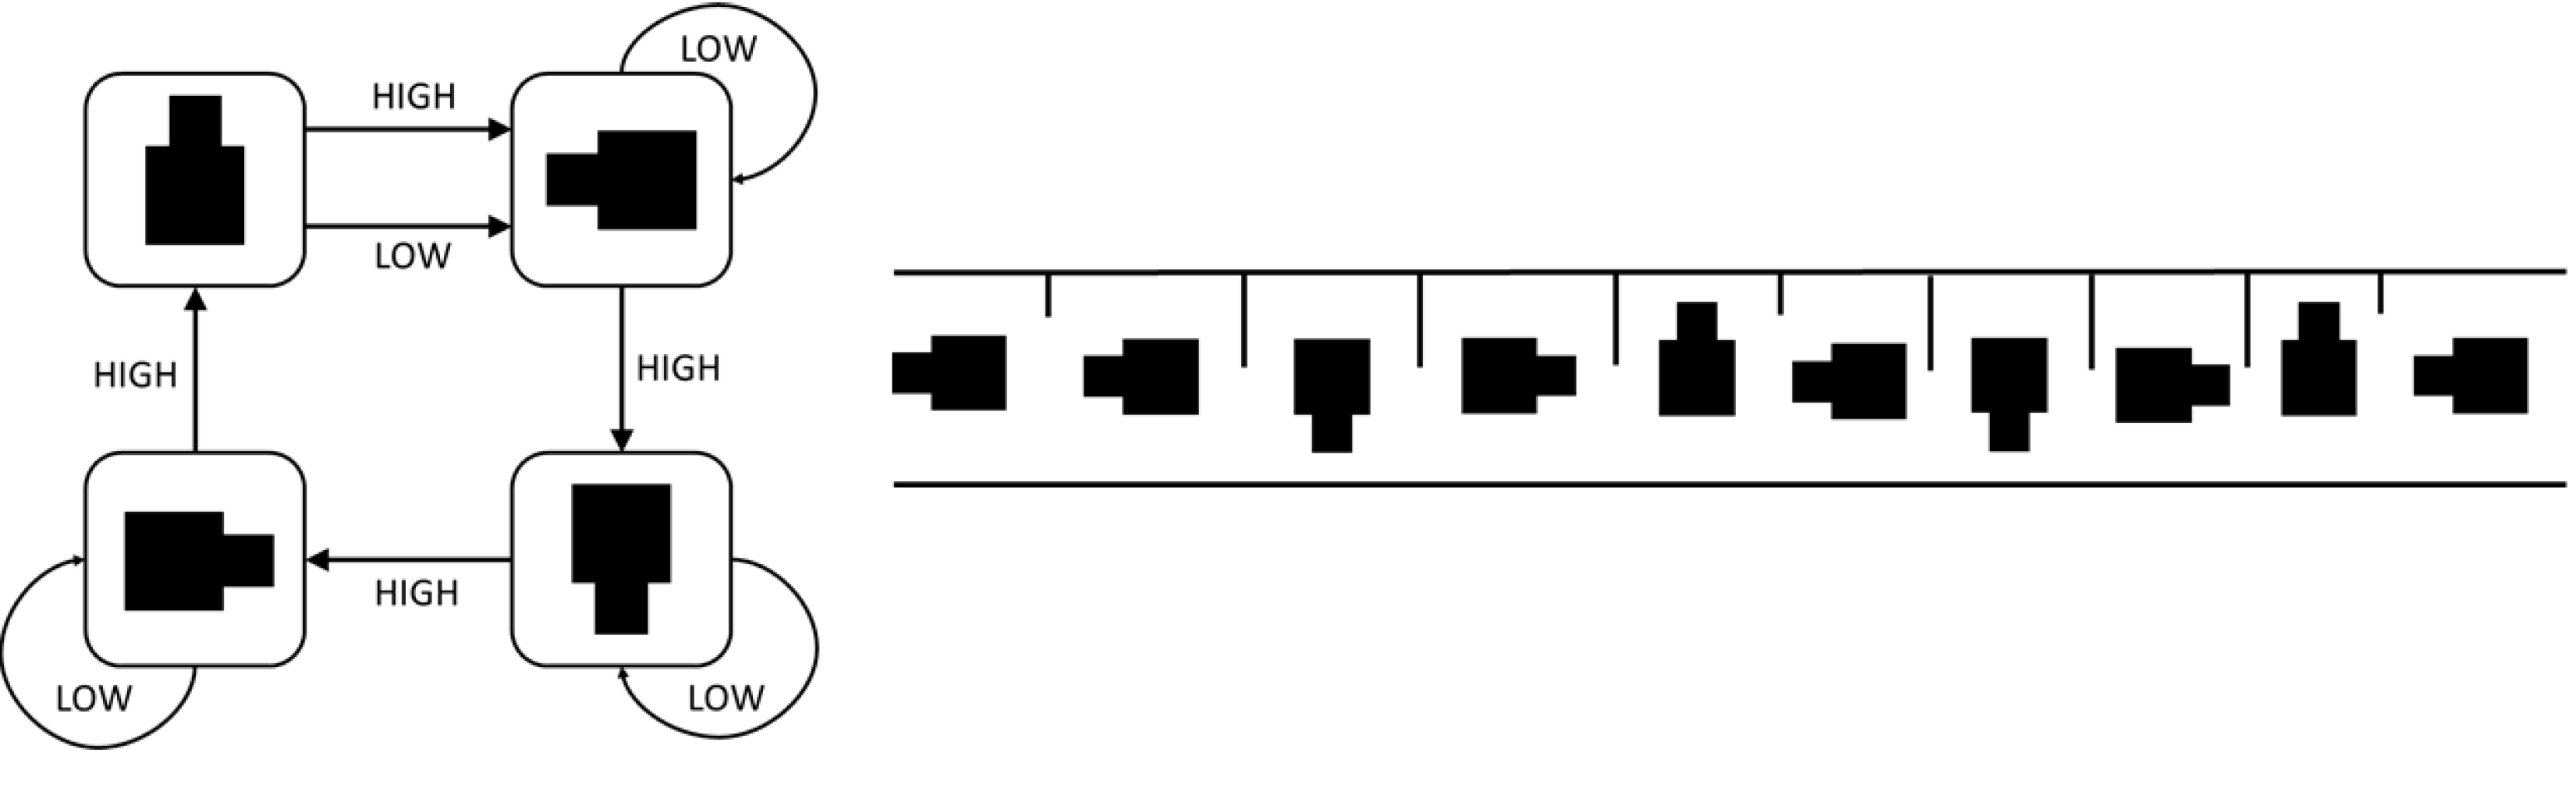
\includegraphics[width=\textwidth]{../part1/sync/part-orienter.png}
\caption[Part orienter problem modeled as a finite automaton]{Left: The part orienter problem modeled as a finite automaton.
	Right: Sequence of effects on one component moving from left to right.		
	Image taken from Podolak et al.~\cite{DBLP:journals/eswa/PodolakRSZ18}. } 
\label{intro:fig:part-orient-solution}	
\end{figure} 

The above scheme works without the use of sensors and does not require any observer or external mechanism to orient the parts. Employing sensorless methods for part orientation is often preferable to using more complicated machinery because of their robustness, simplicity, and ease of maintenance.
In another sensorless approach to part feeding, parts are placed on a vibrating surface and must pass certain obstacles. Such orientation schemes have apparently been employed since the mid-20th century; see~\cite{Sadasivam2015} for a survey on vibratory  part feeders. Sensorless methods for orienting parts without vibrating surfaces were first described by Erdmann and Mason~\cite{DBLP:journals/trob/ErdmannM88}, who simplified and mathematically analyzed a mechanical device originally introduced by Grossman and Blasgen~\cite{DBLP:journals/tsmc/GrossmanB75}.

The first author to investigate the computational complexity of designing sensorless part orienters was Natarajan~\cite{DBLP:conf/focs/Natarajan86,DBLP:journals/ijrr/Natarajan89}. He studied the engineering problem of orienting polygonal objects on conveyor belts using simple, robust, and sensorless methods based on mechanical contact points installed along the belt. Mathematically, he modeled this problem both as a pebbling game and as the problem of finding a sequence of functions from a given set that realizes a constant function. He noted (without proof) 
that a generalization of the latter formulation is \PSPACE-complete and gave polynomial-time algorithms for several variants of these problems.

Natarajan's algorithmic approach to part orienting stimulated substantial
further research in this area. For example,
Goldberg~\cite{DBLP:journals/algorithmica/Goldberg93} introduced a scheme
that orients parts by squeezing them with parallel-jaw grippers and gave a
polynomial-time algorithm for designing a sequence of squeezes that orients
any part, conjecturing that a linear number of squeezes always suffices.
Chen and Ierardi~\cite{DBLP:journals/algorithmica/ChenI95} later confirmed
this conjecture.

Eppstein~\cite{Eppstein90} observed the connection to synchronizing automata previously studied in automata theory, characterized the class of automata investigated by Natarajan~\cite{DBLP:conf/focs/Natarajan86}, and improved Natarajan's algorithms. In this sense, 
synchronizing automata emerged independently in the mechanical engineering literature.
Part orienting as a motivating example for synchronizing automata was later popularized by Ananichev and Volkov~\cite{AnanichevVolkov04,DBLP:journals/tcs/AnanichevV04}; see also the widely cited survey~\cite{DBLP:conf/lata/Volkov08}.

\subsection{Lost in a Maze} 
\label{intro:sec:examples:maze}

Imagine a maze in which every junction has exactly $k$ outgoing corridors
and all junctions look alike, so that a visitor can never tell where they
currently are. The corridors leaving a junction are to be marked with $k$
distinct colors, one color per corridor, and a visitor who is told a
sequence of colors follows the corresponding corridors one after the other.
The task of whoever installs the signs is the following.

\smallskip
\begin{center}
	\fbox{%
		\begin{minipage}{0.9\linewidth}%{\dimexpr\linewidth-2\fboxsep-2\fboxrule\relax}
			Can the corridors be colored so that some sequence of colors
			leads every visitor to one and the same junction, no matter
			where in the maze they started?
		\end{minipage}
	}
\end{center}
\smallskip

Such a sequence does not point at the exit directly; it brings all visitors
to a common junction, and from there a single fixed route takes them out.
Coloring the corridors turns the maze into a deterministic finite automaton:
the junctions are the states, the colors form an alphabet of size $k$, and
a corridor colored~$a$ from junction~$p$ to junction~$q$ gives the
transition $\delta(p,a) = q$. The question above then asks whether the
corridors admit a coloring for which the resulting automaton is
synchronizing.

Not every maze does. If, for instance, the junctions can be split into two
groups such that every corridor leads from one group to the other, then two
visitors starting in different groups stay in different groups forever,
whatever the coloring and whatever sequence they are given. Ruling out
obstructions of this kind is in fact enough: the \emph{road coloring
	theorem}, conjectured by Adler, Goodwyn, and Weiss~\cite{adler77} and proved
by Trahtman~\cite{trahtman09} some thirty years later, states that a
synchronizing coloring exists if and only if the maze is strongly connected
and the lengths of its closed walks have greatest common divisor one.
\IN{road coloring theorem}
\IN{road coloring problem|see{road coloring theorem}}	

\section{Reset Length and the \Cerny Conjecture} 
\label{intro:sec:cerny}

\label{def:rt} 
\label{def:Cn}
\IN{reset length}
\IN{\v{C}ern\'y automata family}
The \emph{reset length} of a synchronizing automaton $\semiautomat{A}{Q}{\Sigma}{\delta}$ is 
\[
\rt{\mathcal A} = \min\{ |u| : u \in \Syn(\mathcal A) \}.
\]
\v{C}ern\'y~\cite{Cer64} proved that, for $n \ge 1$, we have
\[ 
(n-1)^2 \le \max\{ \rt{\mathcal A} \mid \mathcal A \text{ has $n$ states and $\Syn(\mathcal A) \ne \emptyset$} \} \le 2^n - n - 1.
\]
For the lower bound, he gave the
\emph{\Cerny family of automata}
$\mathcal C_n = ([n], \{a,b\}, \delta_n)$
where $n \ge 2$ and
\[
\applytrans{\delta_n}{i}{b} = \begin{cases}
	i + 1 & \text{if } i < n - 1, \\ 
	0     & \text{if } i = n - 1,
\end{cases} 
\qquad
\applytrans{\delta_n}{i}{a} = \begin{cases}
	1  & \text{if } i = 0, \\ 
	i  & \text{if } i \ne 0,
\end{cases}
\]
see \cref{intro:fig:cerny}. The automaton from the part orientation problem in \cref{intro:fig:part-orient-solution}
equals $\mathcal C_4$. Below, we give a proof that $\rt{\mathcal C_n} = (n-1)^2$, 
which also shows that
$(ab^{n-1})^{n-2}a$ is the only shortest synchronizing word for~$\mathcal C_n$.

\begin{figure}[ht]
	\centering	
	\begin{tikzpicture}[shorten >=1pt,->]
		\foreach \name/\angle/\text in {P-n-2/234/n-2, 
			P-n-1/162/n-1, 
			P-0/90/0, 
			P-1/18/1, 
			P-2/-54/2}
		\node[state, minimum size=3.2em] (\name) at (\angle:6em) {$\text$};
		
		\path (P-n-2) edge [left] node {$b$} (P-n-1)
		(P-n-1) edge [above,pos=0.35] node {$b$} (P-0)
		(P-n-1) edge [loop left] node {$a$} ()
		(P-0) edge [above] node {$a,b$} (P-1)
		(P-1) edge [right] node {$b$} (P-2)
		(P-n-2) edge [loop left] node {$a$} ()
		(P-1) edge [loop right] node {$a$} ()
		(P-2) edge [loop right] node {$a$} ();
		
		\node [right = of P-n-2, xshift=-2.5em] {\large $\ldots$};
	\end{tikzpicture}
	\caption[\Cerny family $\mathcal C_n$]{Automata from the \Cerny family $\mathcal C_n$. See \cref{intro:sec:cerny}.}
	\label{intro:fig:cerny}
\end{figure}

%\begin{theorem}%[\Cerny~\cite{Cer64}]
%	\label{intro:cerny_rt}
%	For $n \ge 2$, the unique shortest synchronizing word of $\mathcal C_n$
%	is $(ab^{n-1})^{n-2}a$. Thus $\rt{\mathcal C_n} = (n-1)^2$.
%\end{theorem}
\begin{theorem}[\Cerny~\cite{Cer64}]
	\label{intro:cerny_rt}
	For $n \ge 2$, we have $\rt{\mathcal C_n} = (n-1)^2$.
	Moreover, $(ab^{n-1})^{n-2}a$ is the unique shortest synchronizing word
	of~$\mathcal C_n$.
\end{theorem}
\begin{proof}
	Identify $Q = [n]$ with $\mathbb Z_n$, so that $\applytrans{\delta_n}{p}{b} = p+1$
	(modulo~$n$) for $p \in Q$, while~$a$ maps~$0$ to~$1$ and fixes all other states.
	An \emph{interval} is a non-empty set $[p,q] = \{p, p+1, \ldots, q\}$ with $p,q \in Q$.
	Note that $Q = [p,p-1]$ for every $p \in Q$, and that for $I \ne Q$ the states~$p$
	and~$q$ with $I = [p,q]$ are determined by~$I$, as~$p$ is the only state in~$I$
	with $p - 1 \notin I$ and~$q$ the only one with $q + 1 \notin I$.
	In particular, an interval containing~$1$ but not~$0$ begins at~$1$,
	and an interval containing~$0$ but not~$1$ ends at~$0$.
	\IN{interval} \label{def:interval}
	
	One verifies inductively that $\applytrans{\delta_n}{Q}{(ab^{n-1})^{j}a} = [1,n-1-j]$
	for $0 \le j \le n-2$, so $(ab^{n-1})^{n-2}a$ synchronizes $\mathcal C_n$
	and a shortest synchronizing word exists.
	Let $w = x_1 \cdots x_m$ with $x_1, \ldots, x_m \in \Sigma$ be one
	with $\applytrans{\delta_n}{Q}{w} = \{q\}$ and let
	\[
	I_j = \{\, p \in Q \mid \applytrans{\delta_n}{p}{x_{j+1} \cdots x_m} = q \,\}
	\qquad (0 \le j \le m).
	\]
	Then $I_m = \{q\}$, $I_0 = Q$ and
	$I_{j-1} = \{\, p \in Q \mid \applytrans{\delta_n}{p}{x_j} \in I_j \,\}$ for $j \ge 1$.
	Every state~$p$ satisfies $\applytrans{\delta_n}{p}{x_1 \cdots x_j} \in I_j$;
	in particular, no~$I_j$ is empty.
	Moreover $I_j \ne Q$ for $j \ge 1$, as $I_j = Q$ means that
	$x_{j+1} \cdots x_m$ maps every state to~$q$ and is thus a shorter synchronizing word.
	
	Let $1 \le j \le m$ and assume that~$I_j$ is an interval, say $I_j = [p_j, q_j]$,
	which is possible in a unique way as $I_j \ne Q$.
	Since $\applytrans{\delta_n}{p}{a} \in I_j$ holds for $p \ne 0$ exactly when
	$p \in I_j$, and for $p = 0$ exactly when $1 \in I_j$, exactly one of the following
	cases occurs.
	\begin{enumerate}%[itemsep=0pt, topsep=2pt, parsep=0pt]
		\item $x_j = b$; then $I_{j-1} = [p_j - 1, q_j - 1]$, so $|I_{j-1}| = |I_j|$
		and $p_{j-1} = p_j - 1$.
		
		\item $x_j = a$ and $\{0,1\} \subseteq I_j$ or $\{0,1\} \cap I_j = \emptyset$;
		then $I_{j-1} = I_j$.
		
		\item $x_j = a$ and $0 \in I_j$ but $1 \notin I_j$; then $I_j = [p_j,0]$
		with $p_j \ne 0$ as $I_{j-1} \ne \emptyset$, and
		$I_{j-1} = I_j \setminus \{0\} = [p_j,n-1]$.
		
		\item $x_j = a$ and $1 \in I_j$ but $0 \notin I_j$; then $p_j = 1$,
		and $I_{j-1} = I_j \cup \{0\} = [0,q_j]$, so $|I_{j-1}| = |I_j| + 1$
		and $p_{j-1} = 0 = p_j - 1$.
	\end{enumerate}
	In each case~$I_{j-1}$ is again an interval. So, starting from $I_m = [q,q]$ and
	descending, every~$I_j$ is an interval.
	
	The cases~(2) and~(3) never occur: in both we have $I_{j-1} \subseteq I_j$,
	and, since every state~$p$ satisfies
	$\applytrans{\delta_n}{p}{x_1 \cdots x_{j-1}} \in I_{j-1} \subseteq I_j$ and hence
	$\applytrans{\delta_n}{p}{x_1 \cdots x_{j-1}x_{j+1} \cdots x_m} = q$,
	deleting the letter~$x_j$ from~$w$ leaves a shorter synchronizing word
	in these cases.
	
	Since $|I_m| = 1$ and $|I_0| = n$, the word~$w$ contains exactly $n-1$ letters~$a$.
	Let $j_1 < \cdots < j_{n-1}$ be their positions, so that~$j_1$ is the position of the
	first letter~$a$ in~$w$ and~$j_{n-1}$ that of the last.
	Here $j_1 = 1$, as otherwise $x_1 = b$ and $Q = I_0 = [p_1 - 1, q_1 - 1]$,
	giving $I_1 = Q$, which we excluded;
	and $j_{n-1} = m$, as otherwise $x_m = b$ and $I_{m-1} = \{q-1\}$ by case~(1),
	so that $x_1 \cdots x_{m-1}$ maps every state to $q-1$ and is shorter.
	Now let $2 \le k \le n-1$. The positions~$j$ with $j_{k-1} < j < j_k$ all carry the
	letter~$b$, and by case~(4) we have $p_{j_k - 1} = 0$ and $p_{j_{k-1}} = 1$.
	Since each~$b$ decreases the first state by one and these run from
	$p_{j_k - 1} = 0$ down to $p_{j_{k-1}} = 1$, their number
	$j_k - j_{k-1} - 1$ is congruent to $-1$ modulo~$n$.
	It equals $n-1$, since otherwise it is at least $2n-1$ and deleting $n$ consecutive
	letters~$b$, which changes no transition as $\applytrans{\delta_n}{p}{b^n} = p$,
	would again shorten~$w$. Hence $j_k - j_{k-1} = n$ for all~$k$ and therefore
	\[
	m = \sum_{k=2}^{n-1} (j_k - j_{k-1}) + 1 = (n-2)n + 1 = (n-1)^2 .
	\]
	So the letters~$a$ occupy the positions $1, n+1, \ldots, (n-2)n + 1 = m$, while all
	remaining positions carry the letter~$b$.
	Thus $\rt{\mathcal C_n} = (n-1)^2$ and $w = (ab^{n-1})^{n-2}a$.
\end{proof}

Eppstein~\cite{Eppstein90} introduced the notion of an interval for a more general
class of automata. For a shortest synchronizing word $w = uv$ of $\mathcal C_n$,
he proved $\rt{\mathcal C_n} = (n-1)^2$ by bounding the length of a shortest interval
containing $\delta_n([n],u)$~\cite[Thm.~3]{Eppstein90}, whereas the original proof
by \Cerny~\cite[Lem.~1]{Cer64} considered the length of a largest interval in
$[n] \setminus \delta_n([n],u)$.
The proof above instead uses the sets $\{ p \in [n] \mid \delta_n(p,v) = q \}$,
which are intervals, whenever non-empty, for every word~$v$,
and this also yields the uniqueness asserted in \cref{intro:cerny_rt}.
Salomaa~\cite[Sec.~7]{DBLP:conf/birthday/Salomaa12}
later gave a proof related to \Cerny's
in the form of a solitaire game
in which states are marked by stones
(see also~\cite[Thm.~8]{DBLP:journals/tcs/Salomaa03},
where the argument is adapted to the case in which all states are mapped to a fixed state).
A graph-theoretical proof relating the reset length
to the exponent of certain digraphs was given
by Ananichev et al.~\cite[Thm.~3]{AnaVolGus2013}
(see also~\cite[Prop.~3.1]{KariVolkov2021}).

\IN{\Cerny bound}
\IN{\Cerny conjecture}
In~\cite{DBLP:journals/kybernetika/CernyPR71,Starke66} the authors conjectured the following bound (the so-called \emph{\v{C}ern\'y bound}).

% https://tex.stackexchange.com/questions/102737/how-to-specify-height-and-width-of-fbox
\begin{center} 
	\fbox{\parbox[c]{0.92\textwidth}{\Cerny conjecture: 
			We have $\rt{\mathcal A} \le (n-1)^2$ for every synchronizing $n$-state $\mathcal A$.
	}}
\end{center}

This conjecture, which has remained open for more than five decades, has stimulated extensive research since its formulation.
The reader might wonder why the conjecture is not named after Starke, even though his paper~\cite{Starke66} predates~\cite{DBLP:journals/kybernetika/CernyPR71}.
One possible reason is that older papers often referred only to the seminal work~\cite{Cer64} when discussing the conjecture, despite the fact that, although it introduced synchronizing automata and the \Cerny automata, it did not explicitly state the conjecture itself.
Another possible reason is that \Cerny discussed the conjecture at two conferences shortly after the publication of~\cite{Cer64}.
In any case, even the term ``\Cerny--Starke conjecture'' was never adopted in the literature; see~\cite{DBLP:journals/jalc/Volkov19} for further discussion  on the origin of this conjecture.

\begin{table}[htb]
	\centering
	\caption[Published upper bounds on the reset length]{
		Published upper bounds for the reset length. Kfoury's bound
		was communicated to him by Paterson, see~\cite{Kfoury70}.
		}
	\label{tab:reset_length_bounds}
	
	\begin{tabular}{lll}
		\toprule
		Upper Bound & Remark & Reference \\
		\midrule
		
		$2^n - n - 1$ & & (1964, \Cerny~\cite{Cer64}) \\
		$\tfrac{1}{2}n^3 - \tfrac{3}{2} n^2 + n + 1$ & & (1966, Starke~\cite{Starke66}) \\
		$\tfrac{1}{2} n^3 - n^2 + \tfrac{1}{2} n$ & & (1970, Kohavi~\cite{Kohavi70}) \\
		$\tfrac{1}{3} n^3 - n^2 - \tfrac{1}{3} n + 6$ & & (1970, Kfoury~\cite{Kfoury70}) \\
		$\tfrac{1}{3} n^3 - \tfrac{3}{2} n^2 + \tfrac{25}{6} n - 4$
		& & (1971, \Cerny et al.~\cite{DBLP:journals/kybernetika/CernyPR71}) \\
		
%		$\tfrac{1}{6} n^3 - \tfrac{1}{6} n$
	%	& & (1971, Kohavi and Winograd) \\
		
		$\tfrac{7}{27} n^3 - \tfrac{17}{18} n^2 + \tfrac{17}{6} n - 3$
		& $n = 3k$
		& (1977, Pin~\cite{Pin77a}) \\
		
		$\left(\tfrac{1}{2} + \tfrac{\pi}{36}\right)n^3 + o(n^3)$
		& & (1978, Pin~\cite{Pin81a,DBLP:journals/eik/Pin78,Pin83a}) \\
		
		$\tfrac{1}{6}n^3 - \tfrac{1}{6}n$
		& & (1983, Pin/Frankl~\cite{Frankl82,Pin83a}, 1987, Klyachko et al.~\cite{KlyachkoRystsovSpivak87}) \\		
		$\alpha n^3 + o(n^3)$ & $\alpha \approx 0.1664$ & (2018, Szyku\l a~\cite{szykula2018}) \\
		$\alpha n^3 + o(n^3)$ & $\alpha \le 0.1654$ & (2019, Shitov~\cite{shitov2019}) \\
		
		\bottomrule
	\end{tabular}
\end{table}

\Cref{tab:reset_length_bounds} lists the published upper bounds in chronological order.
Klyachko et al.~\cite{KlyachkoRystsovSpivak87} independently proved the Pin--Frankl bound from \cref{tab:reset_length_bounds} behind the Iron Curtain. Pin~\cite{Pin83a} actually concluded the bound $(n^3 - n)/6 - 1$ for $n \ge 4$
with Frankl's result~\cite{Frankl82}. 
The bound $(n^3 - n)/6$ had previously been stated by Kohavi and Winograd~\cite{KOHAVI1971197,DBLP:journals/jcss/KohaviW73}, yet, somewhat mysteriously, their work was never cited in the subsequent literature. Their argument broadly follows the same approach as that of Pin~\cite{Pin83a}, analyzing traces of $2$-sets in shortest synchronizing words. However, their treatment of certain maximal traces appears to lack sufficient justification, which may explain why their work was largely ignored (for this reason we also left
it out in \cref{tab:reset_length_bounds}).
Additionally, Salomaa~\cite[Thm.~4]{DBLP:journals/tcs/Salomaa03} proved the bound
$\frac{1}{2}n^3 - \frac{3}{2}n^2 + 2n$
for the length of a shortest word mapping all states to a fixed state, rather than merely to some state as required for synchronization.

The \Cerny conjecture~\cite{Cer64} has been confirmed
for a variety of classes of automata, to name a few of them 
(without further explanation and with no claim for completeness):

% https://texfaq.org/FAQ-complist
\begin{enumerate}%[itemsep=-4pt]	
	\item circular automata~\cite{Dubuc96,Dubuc98,DBLP:conf/icalp/Pin78},
	
	\item oriented automata~\cite{Eppstein90}, 
	
	\item (weakly generalized) monotonic automata~\cite{AnanichevVolkov04,DBLP:journals/tcs/AnanichevV04,AnanichevV05}
	and $0$-monotonic automata~\cite{Ananichev2010},
	
	\item automata with a trap state~\cite{DBLP:conf/birthday/Babcsanyi09,Rystsov97},
		
	\item commutative~\cite{DBLP:journals/actaC/ImrehS95,FernauHoffmann19,Rys96}, partially ordered~\cite{Ryzhikov19a}, solvable~\cite{Rystsov97}, and automata whose transition monoid belongs to the varieties \textbf{DS}~\cite{almeida2009representation} or \textbf{EDS}~\cite{AlmeidaS09},
		
	\item strongly reset automata~\cite{Rystsov97}, 
	
	\item nilpotent and (reverse and generalized) definite   automata~\cite{DBLP:journals/actaC/ImrehS95,Rystsov97},
	
	\item automata whose set of synchronizing words is a shuffle ideal~\cite{DBLP:journals/jalc/PetkovicS01},
	
	\item Eulerian automata~\cite{DBLP:journals/tcs/Kari03},
	
	\item automata preserving a chain of partial orders~\cite{DBLP:journals/tcs/Volkov09},
	
	\item automata whose transition monoid contains a $\operatorname{\mathbb{Q} I}$-group~\cite{ArCamSt2017,ArnoldS06},
	
	\item  aperiodic automata~\cite{Trahtman07},
	
	\item automata with a blocking state~\cite{DBLP:conf/birthday/Babcsanyi09},
	%\footnote{\cite[Ex.~4]{DBLP:conf/birthday/Babcsanyi09} should probably read $\delta(n-1,x_n) = n-1$ instead of $\delta(n-1,x_n) = n$.}	
	
	\item automata whose transformation semigroup contains a group fulfilling certain representation-theoretical conditions~\cite{Steinberg10},
		
	\item one-cluster automata with a cycle of prime length~\cite{Steinberg11a},
	
	\item \label{type:genwords} automata $\mathcal A$ with restrictions on generating words for $\Syn(\mathcal A)$~\cite{DBLP:journals/jalc/FrigeriR19,DBLP:journals/iandc/PribavkinaR11},
		
	\item automata that cannot recognize $\{a,b\}^*ab\{a,b\}^*$~\cite{AlmeidaS09},
	
	\item certain aperiodically $1$-contracting automata~\cite{Don16}, 
	
	\item decoder automata for finite maximal prefix codes~\cite{BerlinkovS16},
	
	\item automata having letters of a certain rank~\cite{BerlinkovS16},
	
	\item automata respecting intervals of a digraph~\cite{DBLP:journals/dmtcs/GrechK13a},	

	\item strongly semisimple automata~\cite{DBLP:journals/ijfcs/AlmeidaR16} (related to~\cref{type:genwords}, see also~\cite{Rodaro2019}),
	
	\item automata with two idempotent letters~\cite[Prop.~5]{DBLP:journals/jalc/Volkov19a},
	
	\item $2$-junction automata~\cite{DBLP:journals/dam/GrechK20a},
	
	\item automata with simple idempotents having no permutational letter
	or containing a regular permutation group in the transition monoid~\cite{Rystsov2022},
	
	\item automata for which their sets of synchronizing words have minimal generating words not containing a word of a certain length~\cite{DBLP:journals/jalc/FrigeriR19}, 
		
	\item binary automata with a simple idempotent letter~\cite{volkov2025listresultsvcernyconjecture}, 
	
	\item automata with strongly connected restricted Rystsov graph~\cite{CasasVolkov2024Don,volkov2025listresultsvcernyconjecture},
	
	\item media automata~\cite{Eppstein2007Algorithms},
	
	\item automata without involutions~\cite{Trahtman2008}.
\end{enumerate}

Furthermore, quadratic upper bounds on the reset length have been obtained for automata whose transition monoid contains every transformation~\cite{DBLP:journals/ijfcs/GonzeGJGV19}, for one-cluster automata~\cite{BeaBerPer2011},
for quasi-Eulerian and quasi-one-cluster automata~\cite{DBLP:journals/ijfcs/Berlinkov13},
for regular automata~\cite{Rystsov1995a,Rystsov95a},
for automata with coinciding cycles~\cite{DBLP:conf/dlt/Ruszil23},
for automata with simple idempotents~\cite{Rystsov2000}, for automata having a one-point singular and satisfying additional conditions~\cite{Rystsov2024},\footnote{Both~\cite{AnanichevVolkov04} and~\cite{Rystsov2024} also contain more general formulations of the \Cerny conjecture for transformation monoids.} for automata whose transformation monoid contains a transitive group~\cite{DBLP:conf/fsttcs/000124a}, and for completely reachable automata~\cite{DBLP:conf/icalp/FerensS23}, the latter improving and extending the results of~\cite{DBLP:journals/ijfcs/GonzeGJGV19}. 
For several subclasses of automata, bounds tighter than $(n-1)^2$
are known. For instance, for solvable automata~\cite{Rystsov97}, the bound is $n - 1$. 
A comprehensive overview of such bounds and subclasses can be found in the living list~\cite{volkov2025listresultsvcernyconjecture} of results related to the \Cerny conjecture maintained by Mikhail Volkov.

\chapter{Outline and Contribution}
\label{intro:chap:overview}

First, in \cref{overview:sec:problems} we introduce the two central 
problems with which the thesis is concerned: the constrained
synchronization problem (\cref{overview:sec:csp})
and the description of automata for sets of synchronizing 
words (\cref{intro:overview:structure_set_of_sync_words}).
\Cref{overview:sec:organization} gives an overview on the 
organization of the present work.
Finally, \cref{overview:sec:papers} lists the papers on which this work is based, 
as well as the unpublished results that we have included.

\section{The Problems}
\label{overview:sec:problems}

\subsection{The Constrained Synchronization Problem}
\label{overview:sec:csp}

\IN{constrained synchronization problem} 
\IN{constraint language}
\index{regular constraint language|see{constraint language}}
The \emph{constrained synchronization problem} asks whether a given
deterministic and complete
semiautomaton has  a synchronizing word contained
in a given regular \emph{constraint language}. 
Formally, let~$\Sigma$ be an alphabet 
and $L \subseteq \Sigma^*$ be a regular language 
(see \cref{prelim:sec:decision_problems,prelim:sec:regularlang}
for formal definitions of decision problems and regular languages, respectively).
The problem \constrsync{L} of \emph{constrained synchronization} 
with respect to the \emph{constraint language $L$} is the following decision problem.

\index{\constrsync{L}|see{constrained synchronization problem}}
\begin{center}
\begin{tcolorbox}[width = 0.9\textwidth,colback=white,arc=0pt,outer arc=0pt,boxrule=0.7pt,left =0.5em,right=0em]
\decisionproblem{\constrsync{L}}
{A deterministic and complete semiautomaton $\semiautomat{A}{Q}{\Sigma}{\delta}$.}
{Does there exist a word $w \in L$ synchronizing $\mathcal A$?} 
\end{tcolorbox}
\end{center}

This problem, systematically studied in~\cite{FernauGHHVW19},
firstly appeared in connection with a reduction procedure introduced in~\cite{Gusev2012},
as well as implicitly in reductions used in~\cite{Martyugin14}.
\Cref{constr_sync:sec:motivation} provides further motivation and details.

\subsection{Automata for Sets of Synchronizing Words}
\label{intro:overview:structure_set_of_sync_words}

The set of synchronizing words of a given automaton can be accepted by another automaton of size exponential in the size of the original automaton (see \cref{chap:prelim} for the definition of automata as language acceptors). In this thesis, we also study automata for sets of synchronizing words.
Our motivation comes from the constrained synchronization problem, whose computational complexity is governed by two parameters: the \emph{structure of the constraint language} and the \emph{structure of the set of synchronizing words} of the given input automata.
If an automaton recognizing the set of synchronizing words can be constructed in polynomial time for a class of input automata, then the constrained synchronization problem (with any constraint language) is solvable in polynomial time for this class. An example is the class of commutative automata over a fixed alphabet (see \cref{constr_input:subsec:comm}).
Consequently, \NP- or \PSPACE-hardness results (see \cref{prelim:sec:compl_classes} for definitions of complexity classes) imply that automata for the corresponding sets of synchronizing words cannot, in general, be constructed in polynomial time. 
This motivates our interest in automata 
needing exponentially larger accepting automata for their sets of synchronizing words.

Beyond its connection to the constrained synchronization problem, the study of automata for sets of synchronizing words is also motivated by the following observations.

\begin{enumerate}
\item For known families of \emph{slowly synchronizing automata}, that is, automata whose reset length is close to the \Cerny bound, the minimal automata recognizing their sets of synchronizing words are exponentially larger~\cite{DBLP:journals/corr/Maslennikova14,DBLP:journals/ijfcs/Maslennikova19}. 
This raises the question of whether there is a deeper connection between the reset length of an automaton and the size of a minimal automaton recognizing its set of synchronizing words.

\item The operation that maps a regular language to the set of synchronizing words of its minimal automaton is regularity-preserving and can therefore be studied from the perspective of the state complexity of operations~\cite{GaoMRY17,YuZhuangSalomaa1994}.

\IN{reset complexity} 
\item The class of sets of synchronizing words of automata coincides with the class of regular ideal languages (\cref{prelim:thm:sync_words_is_ideal}). Thus, every regular ideal language can be represented by an automaton having it as its set of synchronizing words. This representation can be exponentially more succinct than a representation by an accepting automaton, 
as witnessed by known families of slowly synchronizing automata~\cite{DBLP:journals/corr/Maslennikova14,DBLP:journals/ijfcs/Maslennikova19}. From the perspective of the descriptional complexity of regular languages, it is therefore natural to investigate those regular ideal languages for which the gap between these two representations is maximal. In automata-theoretic terms, this leads to the study of automata for which minimal automata accepting their sets of synchronizing words are as large as possible.

Furthermore, these observations motivate the definition of the \emph{reset complexity} of a regular ideal language as the size of a smallest automaton having this language as its set of synchronizing words. The \Cerny conjecture is equivalent to the statement that the reset complexity of a regular ideal language is at least the square root of the length of a shortest word in the language, plus one~\cite{DBLP:journals/corr/Maslennikova14,DBLP:journals/ijfcs/Maslennikova19}. 
This yields a language-theoretic approach to the \Cerny conjecture through the investigation of shortest words in regular ideal languages~\cite{DBLP:journals/jalc/FrigeriR25,
	DBLP:journals/jalc/FrigeriR19,
	GusevMP13,
	DBLP:journals/fuin/MaslennikovaR18,
	ReisR16,
	DBLP:journals/aam/Rodaro18}.

	
\item As we will see, our results reveal connections between subset reachability properties,
the size of automata for sets of synchronizing words, and the well-known class of primitive permutation groups.
\end{enumerate}

\section{Organization of the Thesis}
\label{overview:sec:organization}

The thesis consists of four parts.
In \cref{part:intro} we give a short introduction on synchronizing automata
and an overview of the thesis.
\Cref{part:prelim} introduces further notions, automata classes,
and gives preliminary computational complexity results.
A detailed overview is given in \cref{intro:outline:orga:sec:prelim}.
\Cref{part:aut} is concerned with automata accepting the set of synchronizing words of a given automaton and is outlined in \cref{intro:outline:orga:sec:autsync} below.
\Cref{part:constrsync} deals with the constrained synchronization problem
and we give an overview in \cref{intro:outline:orga:sec:csp}.

Parts~\ref{part:aut} and~\ref{part:constrsync} are the main parts.
Unless stated otherwise, all the results stated in these 
parts are due to the author of this thesis.

Historically, and as outlined in \cref{overview:sec:problems}, 
our research on the constrained synchronization problem
led us to investigate automata for sets of synchronizing words.
However, in the present work, we first discuss automata for sets of synchronizing words in \cref{part:aut} before turning to the constrained synchronization problem in \cref{part:constrsync}.
We chose this order of presentation because \cref{part:constrsync} relies on results from \cref{part:aut}, whereas \cref{part:aut} is independent of \cref{part:constrsync}.
Moreover, the study of automata accepting sets of synchronizing words is a natural topic in its own right, 
and we expand it beyond its application to the constrained synchronization problem.

\subsection{Structure of \Cref{part:prelim}: Preliminaries}
\label{intro:outline:orga:sec:prelim}

Here, we introduce further notions in \cref{chap:prelim}. 
In \cref{chap:class-transformations} we investigate classes of transformations.
Permutation groups are investigated in \cref{prelim:sec:permgrp}.
More automata-theoretical notions are given in \cref{prelim:sec:automata}. 
Classes of automata and their properties
are investigated in \cref{chap:classes_aut}.
Computational complexity results on subset mapping problems
in automata with respect to certain subclasses 
are investigated in \cref{chap:prelim_complexity_results}.

Most results in this part are taken from the literature.
Some results on idempotent and one-point singular
transformations from \cref{chap:class-transformations}
are new. The notion of strong $\frac{3}{2}$-connectivity
for digraphs introduced here is new. Further, some results in \cref{chap:classes_aut}
are new, see also \cref{overview:sec:unpublished} for more details.
Some structural results on solvable automata in \cref{prelim:subclasses:solvable}
appear in~\cite{DBLP:journals/jalc/000124}.
\Cref{prelim:sec:automata} on automata theory contains some results
on morphism and quotient automata that we have not seen elsewhere.
The results in \cref{chap:prelim_complexity_results} 
were first presented in~\cite{DBLP:journals/jalc/000124}.

\subsection{Structure of \Cref{part:aut}: Automata for Sets of Synchronizing Words} 
\label{intro:outline:orga:sec:autsync}


\Cref{part:aut} studies automata that accept the set of synchronizing words of a given automaton. 
We derive new notions and conditions related to the size of 
accepting automata for sets of synchronizing words, also giving conditions 
under which minimal automata for such sets have maximal size. 
We further relate our findings to classical automata-theoretic results 
from the field of descriptional complexity.
This part is based on the papers~\cite{DBLP:conf/lata/Hoffmann21,
	DBLP:journals/tcs/Hoffmann21,
	DBLP:conf/lata/Hoffmann21a,
	DBLP:conf/dcfs/Hoffmann21,
	DBLP:conf/dcfs/Hoffmann22,
	HoffmannCircularExtended,
	HoffmannLATAextended2,
	Hoffmann2024}, 
but the presentation has been extended and unified, with additional new results included.

Except in \cref{sync_max:sec:compl_reach,sync_max:sec:BVC-graphs,sync_max:sec:augmentative,sync_max:sec:rystsov_graph} and the discussion sections, which review notions and results from the literature, all results presented are novel and due to the author. Next, we describe the organization of \cref{part:aut} and give a broad overview of each chapter and its relation to the work on which this thesis is based. A more detailed overview of the chapters, including descriptions of their individual sections, is given at the beginning of each chapter.

In \cref{sync_max:chap:prelim}, we first note that the set of synchronizing words is a regular language acceptable by the power automaton.
To obtain lower bounds on the size of automata accepting the set of synchronizing words, we apply minimality conditions to the power automaton. This leads us to the notions of reachability of subsets and distinguishability of pairs of subsets.
The rest of the chapter investigates these two notions, giving sufficient conditions for reachability and distinguishability. We also introduce completely reachable automata, a class previously studied in the literature, and the new class of completely distinguishable automata, for which we prove several equivalent characterizations.
The results in this chapter are based on~\cite{DBLP:conf/dlt/Hoffmann23,Hoffmann2024}, where completely distinguishable automata were introduced, but it also contains new unpublished material, see \cref{overview:sec:unpublished}.

\Cref{sync_max:chap:sync_max} introduces sync-maximal automata as synchronizing automata for which an automaton accepting the set of synchronizing words is as large as possible, i.e., for which the gap between the state complexity and the reset complexity of the set of synchronizing words is maximal. We investigate sufficient conditions and derive structural properties, showing that sync-maximal automata are closely related to completely reachable automata. We also give various examples. The notion of sync-maximal automata, as well as the structural results, were first introduced in~\cite{DBLP:conf/dlt/Hoffmann23,Hoffmann2024}. 

\Cref{sync_max:chap:graphs} discusses graph-theoretical constructions that yield sufficient conditions for complete reachability and complete distinguishability. First, we review constructions and results from the literature. We then extend some of these constructions to arbitrary transformation semigroups. Finally, we give graph-theoretical conditions ensuring complete reachability or distinguishability of certain pairs of subsets. The results from this chapter are new and have not been published before.

\Cref{sync_max:sec:subclasses} investigates the following subclasses of automata: commutative automata, automata in which every letter has defect at most one, SI-automata, and circular automata.
For commutative automata, we show that an automaton recognizing the set of synchronizing words can be computed in polynomial time when the alphabet is fixed. This result was published in~\cite{DBLP:journals/tcs/Hoffmann21} in the context of the constrained synchronization problem for commutative constraint languages, and will be used later in \cref{part:constrsync}.
We then consider automata in which every letter has defect at most one. In this setting, we show that if the group of units of the transformation monoid is transitive, then synchronizability implies complete distinguishability. As a consequence, a binary automaton with at least three states is completely reachable if and only if it is sync-maximal. These results are taken from~\cite{Hoffmann2024}.
Then we investigate SI-automata. For example,
we show that in synchronizing SI-automata
distinct pairs $2$-sets are distinguishable.
We derive this from more general and unpublished results,
but it also follows from~\cite[Lem.~11]{DBLP:conf/dcfs/Hoffmann22}.
However, the paper~\cite{DBLP:conf/dcfs/Hoffmann22} 
contains a mistake stemming from a false statement~\cite[Prop.~2]{DBLP:conf/dcfs/Hoffmann22}.
We discuss this in detail at the end of \cref{sync_max:sec:subclasses:discussion}.
Lastly, we investigate circular automata and state a sufficient condition for complete reachability and complete distinguishability. A special case of this condition was published in~\cite{HoffmannCircularExtended}, with a preliminary version presented in~\cite{DBLP:conf/lata/Hoffmann21a}.

\Cref{sync_max:chap:decision} studies the decision problems for complete reachability, complete distinguishability, and sync-maximality, as well as related questions.
For example, we prove that these problems 
are \NL-hard for SI-automata, with complete reachability even being \NL-complete for SI-automata,
and in \PSPACE\ for general automata.
The results on SI-automata were published in~\cite{DBLP:conf/dlt/Hoffmann23,Hoffmann2024}.

\Cref{sync_max:sec:perm_grps} 
discusses relations to permutation groups.
We introduce primitive groups and
characterize them in terms of complete reachability,
complete distinguishability, and in terms of sync-maximality
of associated automata.
The relation of primitive groups to complete reachability
was first published in~\cite{DBLP:conf/lata/Hoffmann21},
and the relation to sync-maximality in~\cite{DBLP:conf/dcfs/Hoffmann21}.
The extended journal publication~\cite{HoffmannLATAextended2} 
of~\cite{DBLP:conf/lata/Hoffmann21,DBLP:conf/dcfs/Hoffmann21} contains 
both of these characterizations.
We then introduce $A$-primitivity 
and study its connection to congruences, orbitals,
generating sets, synchronization, reachability,
and homogeneity properties.
Our results generalize existing characterizations
of primitivity from the literature,
and a characterization by
a homogeneity property also gives
a new characterization. 
The notion of $A$-primitivity is introduced here for the first time, and the results of this chapter have not been published previously.

\Cref{sync_max:chap:slowly} discusses families of slowly synchronizing
automata. We observe that, for most of these families of automata,
the minimal automata accepting their sets of synchronizing words
have exponential size. In particular,
we use results from Chapter~\ref{sync_max:sec:subclasses}
on circular automata to deduce sync-maximality
for several families of slowly synchronizing circular automata
from the literature, including one family for which 
sync-maximality has previously only been conjectured.
This confirmation of the conjecture was 
presented in~\cite{DBLP:conf/lata/Hoffmann21a,HoffmannCircularExtended}.
We then show, for three families of slowly synchronizing but not sync-maximal
automata, that minimal automata for their sets 
of synchronizing words are exponentially larger.
Based on our observations, we formulate various conjectures.
Apart from the confirmation of the aforementioned conjecture,
the results from this chapter have not been published.

\subsection{Structure of \Cref{part:constrsync}: The Constrained Synchronization Problem}
\label{intro:outline:orga:sec:csp}

\Cref{part:constrsync} deals with the constrained synchronization problem and is based on the works~\cite{FernauGHHVW19,
	DBLP:conf/cocoon/Hoffmann20,
	DBLP:conf/ictcs/Hoffman20,
	DBLP:conf/fct/Hoffmann21,
	DBLP:journals/tcs/Hoffmann21,
	DBLP:conf/cocoon/Hoffmann21,
	DBLP:conf/wia/Hoffmann22,
	HoffmannCocoonExtended}.
The results from~\cite{DBLP:conf/cocoon/Hoffmann20,DBLP:conf/fct/Hoffmann21,DBLP:journals/tcs/Hoffmann21,DBLP:conf/cocoon/Hoffmann21,HoffmannCocoonExtended}
were revisited with an emphasis on a more streamlined, coherent, and simplified presentation.
This was achieved primarily through the use of general methods introduced in~\cite{DBLP:conf/cocoon/Hoffmann21,HoffmannCocoonExtended}.

In \cref{constr_sync:sec:motivation}, we give motivational examples for the constrained synchronization problem.

\Cref{constr_sync:chap:further_notions} introduces additional notions that we will need in \cref{part:constrsync}. We also present a new characterization of solid codes that, to the best of our knowledge, has not been published before.

\Cref{constr_sync:chap:gen_results} presents general results on manipulating constraint languages while preserving
the complexity or to deduce complexity lower bounds. Furthermore, we give sufficient conditions for \NP- and \PSPACE-hardness. 
Some of these results
were presented in~\cite{DBLP:conf/cocoon/Hoffmann21,HoffmannCocoonExtended},
which generalized results from~\cite{FernauGHHVW19},
and some results are new.

The central question investigated in \cref{constr_sync:chap:classes_constraint_languages}
is the computational complexity of \constrsync{L} for different classes of regular
constraint languages $L \subseteq \Sigma^*$.
While a complete classification remains an \emph{open problem},
we present several partial results by giving complete classifications for the following classes of constraint languages:
letter-bounded languages, languages accepted by partial automata (PDFAs, introduced in
\cref{constr_sync:chap:further_notions}) with at most two states over an arbitrary alphabet and at most three states over a binary alphabet, and commutative languages.
We also obtain results for infinite, sparse, and monoid languages, as well as
for languages accepted by strongly connected PDFAs.
The classification for commutative constraint languages appeared
in~\cite{DBLP:conf/cocoon/Hoffmann20,DBLP:journals/tcs/Hoffmann21}.
Here, we present a simplified formulation and proof.
The results for sparse and letter-bounded languages appeared
in~\cite{DBLP:conf/ictcs/Hoffman20,DBLP:conf/fct/Hoffmann21}.

Lastly, motivated by the question of what features are needed in input automata to realize certain computational complexities, in \cref{constr_sync:chap:constr_input} we investigate specific types of input automata. Some of the results from this chapter appeared in~\cite{DBLP:conf/wia/Hoffmann22}, and some mistakes from this paper have been corrected.

\section{Work by the Author Relevant to the Thesis}
\label{overview:sec:papers} 

\subsection{Published Work}

The present thesis contains and extends material from the following papers and conference contributions published since 2019, in which the author was involved.

\begin{enumerate}
	\item[\cite{FernauGHHVW19}] \fullcite{FernauGHHVW19}
	\item[\cite{DBLP:conf/ictcs/Hoffman20}] \fullcite{DBLP:conf/ictcs/Hoffman20}
	\item[\cite{DBLP:conf/cocoon/Hoffmann20}] \fullcite{DBLP:conf/cocoon/Hoffmann20}
	\item[\cite{DBLP:conf/lata/Hoffmann21a}] \fullcite{DBLP:conf/lata/Hoffmann21a}
	\item[\cite{DBLP:conf/lata/Hoffmann21}] \fullcite{DBLP:conf/lata/Hoffmann21}
	\item[\cite{DBLP:conf/cocoon/Hoffmann21}] \fullcite{DBLP:conf/cocoon/Hoffmann21}
	\item[\cite{DBLP:conf/dlt/Hoffmann21a}] \fullcite{DBLP:conf/dlt/Hoffmann21a}
	\item[\cite{DBLP:journals/tcs/Hoffmann21}] \fullcite{DBLP:journals/tcs/Hoffmann21} 
	(extended version of~\cite{DBLP:conf/cocoon/Hoffmann20})
	\item[\cite{DBLP:conf/fct/Hoffmann21}] \fullcite{DBLP:conf/fct/Hoffmann21}
	\item[\cite{DBLP:conf/dcfs/Hoffmann21}] \fullcite{DBLP:conf/dcfs/Hoffmann21}
	\item[\cite{DBLP:conf/dcfs/Hoffmann22}] \fullcite{DBLP:conf/dcfs/Hoffmann22}
	\item[\cite{DBLP:conf/wia/Hoffmann22}] \fullcite{DBLP:conf/wia/Hoffmann22}
	%\item[\cite{DBLP:conf/wia/Hoffmann22extended}] \fullcite{DBLP:conf/wia/Hoffmann22extended}
	%(extended version of~\cite{DBLP:conf/wia/Hoffmann22})
	\item[\cite{HoffmannCocoonExtended}] \fullcite{HoffmannCocoonExtended} 
	(extended version of~\cite{DBLP:conf/cocoon/Hoffmann21})
	
	%{\sloppy 
		
	\item[\cite{HoffmannLATAextended2}] \fullcite{HoffmannLATAextended2}
	(extended version of~\cite{DBLP:conf/lata/Hoffmann21})
		
		%\fussy}
	\item[\cite{HoffmannCircularExtended}] \fullcite{HoffmannCircularExtended}
	(extended version of~\cite{DBLP:conf/lata/Hoffmann21a})
	
	\item[\cite{DBLP:conf/dlt/Hoffmann23}] \fullcite{DBLP:conf/dlt/Hoffmann23}
	
	\item[\cite{Hoffmann2024}] \fullcite{Hoffmann2024}
	(extended version of~\cite{DBLP:conf/dlt/Hoffmann23})
	
	\item[\cite{DBLP:journals/jalc/000124}] \fullcite{DBLP:journals/jalc/000124}
\end{enumerate}

\subsection{Unpublished Work} 
\label{overview:sec:unpublished}

Here, we discuss results contained in the present thesis that were not published before.

In~\cref{part:prelim}, the results on one-point singulars 
from~\cref{prelim:sec:oneattractor,prelim:sec:idempotentoneattractor}
are new. We were also unable to find the statements 
from~\cref{prelim:sec:idempotent} on compositions
of idempotent transformations in the literature (but most of them are rather technical or perhaps folklore). We also note that our treatment of automata theory in \cref{prelim:sec:automata}, tailored to our needs, 
differs from those found in the literature of which we are aware,
in particular in its usage of the reachability order
and morphisms. Furthermore, many results related to morphisms
and isomorphisms between automata that
we give are new or scattered throughout the literature under different terminology and notation.

In~\cref{part:aut}, the results on reachable subsets from \cref{sync_max:sec:reachable},
on pairs of distinguishable subsets from~\cref{sync_max:sec:pairs_k_k-1,sync_max:sec:shortestdist},
the graph-theoretical results from~\cref{sec:extended_Rystsov_graph}, 
on automata where every letter has defect at most one from~\cref{sync_max:sec:defectone},
and on subset mapping properties for pairs
of equal-sized sets in SI-automata from~\cref{sec:SI:dist} are new (but one preliminary 
result appeared in~\cite[Lem.~11]{DBLP:conf/dcfs/Hoffmann22}).
Furthermore, the notion of $A$-primitivity is novel
and all results from~\cref{sec:A-primitive} 
appear in this thesis for the first time.

In~\cref{part:constrsync}, some characterizations
of solid codes from \cref{constrsync:sec:codes:solid} are (to the best of our knowledge) new.
The complexity lower bounds involving concatenations from \cref{constr_sync:subsec:concat} have not been published previously.
In \cref{constr_sync:chap:constr_input} some published results have
been corrected or extended. 
For example, the classification for partially ordered automata in \cref{constrinput:sec:two-state-pto} refines the results of~\cite{DBLP:conf/dlt/Hoffmann21a}; the bound for monotonic automata claimed in \cref{constr_sync:prop:monotonic_bound} corrects that of~\cite{DBLP:conf/wia/Hoffmann22}; and the claims on solvable automata in \cref{constr_input:subsec:solvable} have likewise been corrected. See \cref{constr_input:sec:discussion} for details.
Also, some material has been presented differently. Further details on new, extended, or revised material are given in the discussion section at the end of each chapter.
